Crystal symmetry and soft phonon modes.

\begin{parts}
	\part Sketch of lattice in cubic phase:
	\begin{figure}[H]
		\centering
		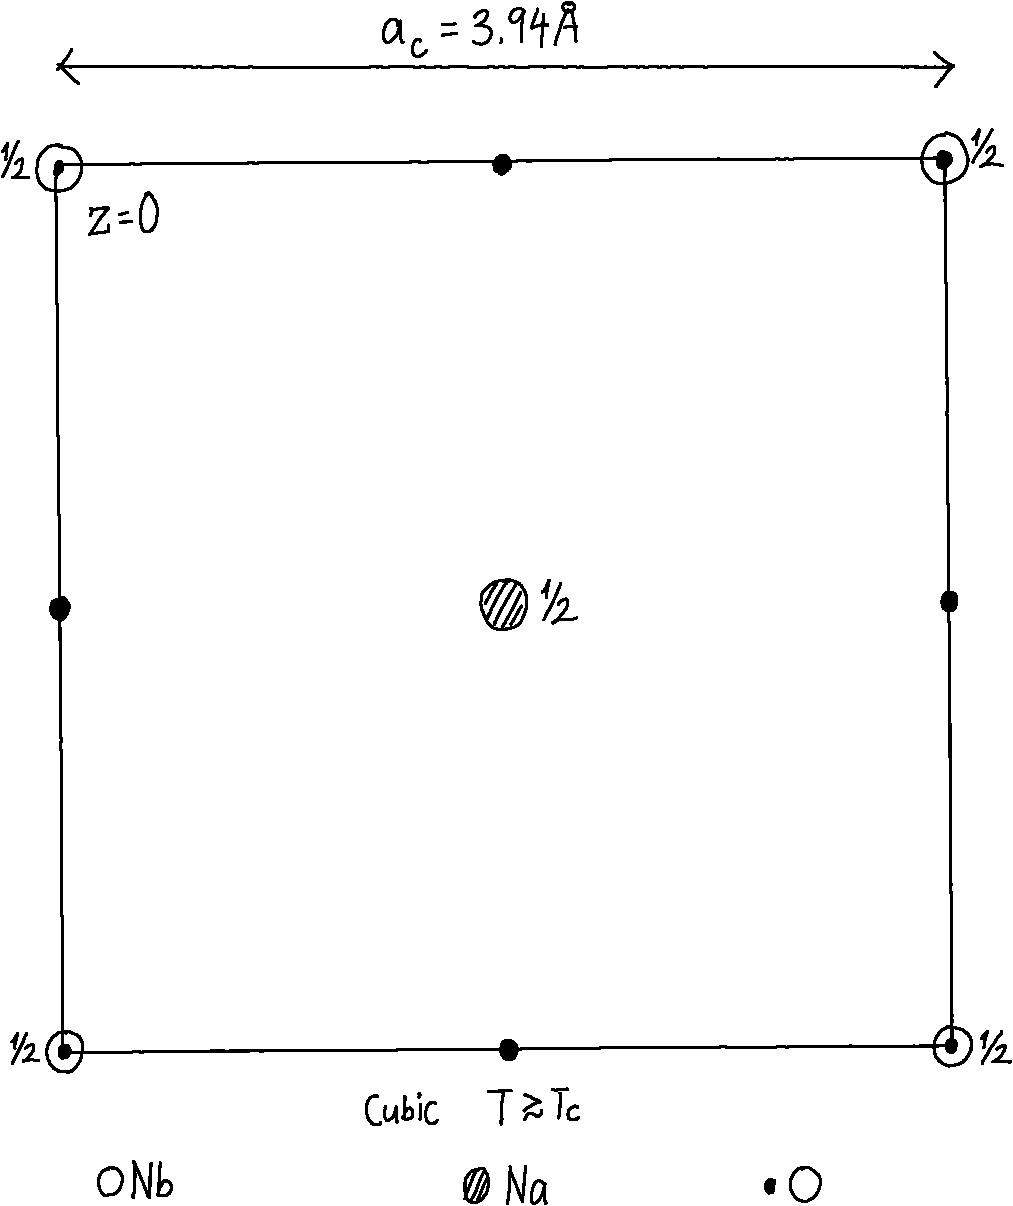
\includegraphics[width=.95\linewidth]{q2-lattice-cubic}
	\end{figure}
	
	\newpage
	Sketch of lattice in tetragonal phase:
	\begin{figure}[H]
		\centering
		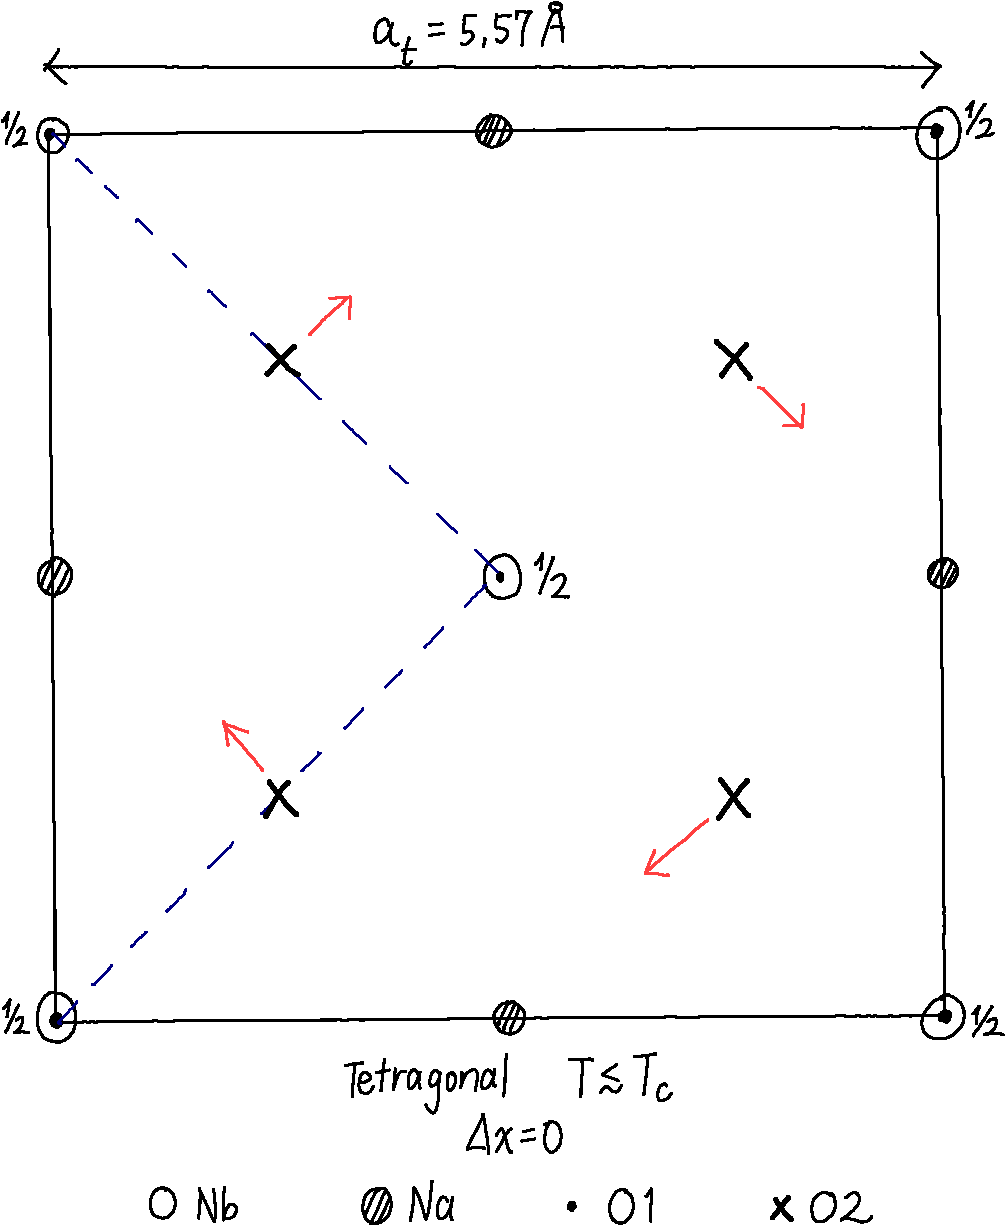
\includegraphics[width=.95\linewidth]{q2-lattice-tetragonal}
	\end{figure}
	
	Note that the cubic UC has rotated $45\degree$ to make the new tetragonal UC (see dashed lines).
	So we have $\mathbf{a}_t = \mathbf{a}_c - \mathbf{b}_c$, $\mathbf{b}_t = \mathbf{a}_c + \mathbf{b}_c$, $\mathbf{c}_t = \mathbf{c}_c$.
	
	\part
	\begin{align*}
		S_\textnormal{Na} &= f_\textnormal{Na} \sbracket{\mathrm{e}^{i2\pi\rbracket{0 + k/2 + l/2}} + \mathrm{e}^{i2\pi\rbracket{h/2 + 0 + l/2}}} \\
		&= f_\textnormal{Na} \mathrm{e}^{i\pi l} \sbracket{\mathrm{e}^{i\pi k} + \mathrm{e}^{i\pi h}}
	\end{align*}
	So Na needs $k$ and $h$ to be both odd/even to have non-zero $S$.
	
	\begin{align*}
		S_\textnormal{Nb} &= f_\textnormal{Nb} \sbracket{\mathrm{e}^{i0} + \mathrm{e}^{i2\pi\rbracket{h/2 + k/2 + 0}}} \\
		&= f_\textnormal{Nb} \sbracket{1 + \mathrm{e}^{i\pi\rbracket{h+k}}}
	\end{align*}
	Selection rule for Nb: $h+k=$ even.
	
	\begin{align*}
		S_\textnormal{O1} &= f_\textnormal{O} \sbracket{\mathrm{e}^{i2\pi\rbracket{0 + 0 + l/2}} + \mathrm{e}^{i2\pi\rbracket{h/2 + k/2 + l/2}}} \\
		&= f_\textnormal{O} \mathrm{e}^{i\pi l} \sbracket{1 + \mathrm{e}^{i\pi\rbracket{h+k}}}
	\end{align*}
	So O1 has the same selection rule as Nb.
	
	\begin{align*}
		S_\textnormal{O2} &= f_\textnormal{O} \sbracket{\mathrm{e}^{i2\pi\rbracket{h/4 + \underbracket{3k/4}_{-k/4} + 0 + h\Delta x + k\Delta x}} + \mathrm{e}^{i2\pi\rbracket{-h/4 + k/4 + 0 - h\Delta x - k\Delta x}} + \mathrm{e}^{i2\pi\rbracket{h/4 + k/4 + 0 - h\Delta x + k\Delta x}} \right. \\
		&\left. \hspace{2em} + \mathrm{e}^{i2\pi\rbracket{\underbracket{3h/4}_{-h/4} - k/4 + 0 + h\Delta x - k\Delta x}}} \\
		&= f_\textnormal{O} \sbracket{2\cos\rbracket{\frac{h-k}{2} + 2(h+k)\Delta x}\pi + 2\cos\rbracket{\frac{h+k}{2} + 2(-h+k)\Delta x}\pi}
	\end{align*}
	\begin{subparts}
		\subpart Note that for $h$ odd, $k$ even (or vice versa), $S_\textnormal{Na} = S_\textnormal{Nb} = S_\textnormal{O1} = 0$, however $S_\textnormal{O2} \neq 0$ if $\Delta x \neq 0$.
		So this family of reflections shall be exclusive to O2 for $\Delta x \neq 0$.
		
		\subpart Also since the lattice is tetragonal, for the parity between $h$ and $k$ to differ, it is also subject to further constraints of $h \neq 0$, $k \neq 0$.
	\end{subparts}
	
	\part For $(2, 1, 0)$, we have $S_\textnormal{Na} = S_\textnormal{Nb} = S_\textnormal{O1} = 0$ from b.
	
	So we have:
	\begin{align*}
		I(2, 1, 0) &\propto \abs{S_\textnormal{O2}}^2 \times M_{(2, 1, 0)} \\
			&= 4f_\textnormal{O}^2 \sbracket{\cos\rbracket{\frac{1}{2} + 6\Delta x}\pi + \cos\rbracket{\frac{3}{2} - 2\Delta x}}^2 \times 8
	\end{align*}
	
	For $(0, 0, 1)$:
	\begin{align*}
		S_\textnormal{Na} &= f_\textnormal{Na} \rbracket{-1} \rbracket{1+1} = -2f_\textnormal{Na} \\
		S_\textnormal{Nb} &= f_\textnormal{Nb} \rbracket{1+1} = 2f_\textnormal{Nb} \\
		S_\textnormal{O1} &= f_\textnormal{O} \rbracket{-1} \rbracket{1+1} = -2f_\textnormal{O} \\
		S_\textnormal{O2} &= 2f_\textnormal{O} \sbracket{\cos 0 + \cos 0} = 4f_\textnormal{O} \\
		\Rightarrow I(0, 0, 1) &\propto \abs{\sum S}^2 \times M_{(0, 0, 1)} \\
		&= 2^2 \rbracket{-f_\textnormal{Na} + f_\textnormal{Nb} + f_\textnormal{O}}^2 \times 2
	\end{align*}
	
	Hence:
	\begin{align*}
		\frac{I(2, 1, 0)}{I(0, 0, 1)} &= \frac{4f_\textnormal{O}^2}{\rbracket{-f_\textnormal{Na} + f_\textnormal{Nb} + f_\textnormal{O}}^2} \sbracket{\cos\rbracket{\frac{1}{2} + 6\Delta x}\pi + \cos\rbracket{\frac{3}{2} - 2\Delta x}}^2 \\
		&= A \sbracket{\cos\frac{\pi}{2} \cos 6\pi\Delta x - \sin\frac{\pi}{2} \sin 6\pi\Delta x + \cos\frac{3\pi}{2} \cos 2\pi\Delta x + \sin\frac{3\pi}{2} \sin 2\pi\Delta x}^2 \\
		&= A \sbracket{\sin 2\pi\Delta x + \sin \underbracket{6\pi\Delta x}_{m = 3}}^2
	\end{align*}
	
	where
	\begin{align*}
		A &= \frac{4f_\textnormal{O}^2}{\rbracket{-f_\textnormal{Na} + f_\textnormal{Nb} + f_\textnormal{O}}^2} \\
		&= \num{0.178} \mtext{assuming $f_X \propto Z_X$ the atomic number of $X$}
	\end{align*}
	
	If neutrons are used instead, the factor $A$ would be in terms of the scattering length $b_X$, which varies rather unpredictably between elements.
	
	\part
	\begin{align*}
		\mathbf{a}_t^* &= \frac{2\pi}{V_t} \mathbf{b}_t \times \mathbf{c}_t \\
		&= \frac{2\pi}{V_t} \rbracket{\mathbf{a}_c + \mathbf{b}_c} \times \mathbf{c}_c \\
		&= \frac{2\pi}{V_t} \rbracket{-\frac{\mathbf{b}_c^*}{2\pi} + \frac{\mathbf{a}_c^*}{2\pi}} \cdot V_c
	\end{align*}
	\begin{align*}
		\mathbf{b}_t^* &= \frac{2\pi}{V_t} \mathbf{c}_t \times \mathbf{a}_t \\
		&= \frac{2\pi}{V_t} \mathbf{c}_c \times \rbracket{\mathbf{a}_c - \mathbf{b}_c} \\
		&= \frac{2\pi}{V_t} \rbracket{\frac{\mathbf{b}_c^*}{2\pi} + \frac{\mathbf{a}_c^*}{2\pi}} \cdot V_c
	\end{align*}
	\begin{align*}
		\mathbf{c}_t^* &= \frac{2\pi}{V_t} \mathbf{a}_t \times \mathbf{b}_t \\
		&= \frac{2\pi}{V_t} \rbracket{\mathbf{a}_c - \mathbf{b}_c} \times \rbracket{\mathbf{a}_c + \mathbf{b}_c} \\
		&= \frac{2\pi}{V_t} \rbracket{2 \mathbf{a}_c \times \mathbf{b}_c} \\
		&= \frac{2\pi}{V_t} \cdot 2 \mathbf{c}_c^* \cdot \frac{V_c}{2\pi}
	\end{align*}
	where $V_c$ is the volume of the tetragonal UC = $2V_c$ that of cubic UC.
	
	Therefore:
	\begin{align*}
		\mathbf{a}_t^* &= \rbracket{\mathbf{a}_c^* - \mathbf{b}_c^*} \times \frac{1}{2} \\
		\mathbf{b}_t^* &= \rbracket{\mathbf{a}_c^* + \mathbf{b}_c^*} \times \frac{1}{2} \\
		\mathbf{c}_t^* &= \mathbf{c}_c^*
	\end{align*}
	Note that the only high symmetry point intersected by $\mathbf{a}_t^*$ and $\mathbf{b}_t^*$ is M, so $\mathbf{k}_s$ is M.
\end{parts}